% main.tex
% Universitaire Papers - Full Documentation & Usage Guide
% Author: Matt
% Purpose: A self-contained manual that explains paperSettings.tex,
%          standardCommands.tex and demonstrates how to use the macros.
%
% Save this file as main.tex in the root of the repo alongside:
%   - paperSettings.tex
%   - standardCommands.tex
%   - main.bib
%
% Compile with: buildLatexDocument.sh (or fullBuild.sh)
% Or upload to Overleaf and compile there.
% -----------------------------------------

% ----------- Document settings -----------
\documentclass[nonacm, sigconf, balance=true]{acmart}
\include{core/paperSettings} % import custom general paper settings
\include{core/standardCommands} % import custom commands and packages
% -----------------------------------------
\begin{document}

    \begin{SimpleTable}[s{1}s{.3}s{.3}]{}{}
        \TableHeader{TERM & LATEX & LATEX COMMAND}
        \TableRow{1. there exists at least one & \exists & \verb|\exists|}
        \TableRow{2. there exists one and only one & \exists! & \verb|\exists!|}
        \TableRow{3. there is no & \nexists & \verb|\nexists|}
        \TableRow{4. for all & \forall & \verb|\forall|}
        \TableRow{5. not (logical not) & \neg & \verb|\neg|}
        \TableRow{6. or (logical or) & \lor & \verb|\lor|}
        \TableRow{7. division & \div & \verb|\div|}
        \TableRow{8. and (logical and) & \land & \verb|\land|}
        \TableRow{9. implies & \implies & \verb|\implies|}
        \TableRow{10. right implication & \Rightarrow & \verb|\Rightarrow|}
        \TableRow{11. is implied by (only if) & \Longleftarrow & \verb|\Longleftarrow|}
        \TableRow{12. left implication & \Leftarrow & \verb|\Leftarrow|}
        \TableRow{13. if and only if, iff & \iff & \verb|\iff|}
        \TableRow{14. equivalence & \Leftrightarrow & \verb|\Leftrightarrow|}
        \TableRow{15.Subset & \subset & \verb|\subset|}
        \TableRow{16. Logical XOR (exclusive or) & \oplus & \verb|\oplus|}
        \TableRow{17. Union of sets & \cup & \verb|\cup|}
        \TableRow{18. Empty set & \emptyset & \verb|\emptyset|}
        \TableRow{19. Intersection of sets & \cap & \verb|\cap|}
        \TableRow{20. Union of sets & \cup & \verb|\cup|}
    \end{SimpleTable}

    \clearpage
    \onecolumn


    \section{Propositielogica}
    Propositielogica is de studie van bewijzen. Een propositie is te beantwoorden met waar of niet waar

    \subsection{Proposities}
    We gebruiken in logica variabelen zoals P en Q, dit zijn \textit{atomisch} proposities, deze zijn altijd geschreven in HOOFDLETTERS.
    Deze zijn niet verder op te delen, dus niet opgebouwd van kleinere delen zoals implicaties etc. deze waardes zijn Waar/True/1 of Onwaar/False/0.

    Je hebt ook kleine letters p, q, \ldots, dit zijn niet-atomische proposities, het zijn geen propositionele formules, maar eerder \textit{metavariabelen}.

    \begin{multicols}{2}

        Elke propositionele formule bestaat uit:
        \begin{itemize}
            \item Atomitsche proposities (P, Q, R, \ldots)
            \item true, (T, Waar, 1)
            \item false, (F, Onwaar, 0)
        \end{itemize}

        Deze kunnen ook kleiner opgedeeld zijn, dan zijn dit ook propositionele formules:
        \begin{itemize}
            \item $P \implies Q$ - \textbf{implicatie} als P, dan Q
            \item $P \land Q$ - \textbf{conjunctie} P én Q
            \item $P \lor Q$ - \textbf{disjunctie} P of Q
            \item $\neg P$ - \textbf{negatie} (niet P / P houd geen stand)
        \end{itemize}

    \end{multicols}

    Zoals in de wiskunde ook is heeft propositielogica óók een volgorde, deze is:
    \begin{enumerate}
        \item Haakjes ()
        \item Negatie $\neg$
        \item Conjunctie $\land$
        \item Disjunctie $\lor$
        \item Implicatie $\implies$
    \end{enumerate}

    $\neg P \lor Q \implies Q \land P$ moet gelezen worden als $((\neg P) \lor Q) \implies (Q \land P)$

    Om dit te onthouden kan je deze zij onthouden: ``Hoe Navigeert Connie De Ijssel''

    \subsection{Semantiek van propositie operatoren}

    \begin{SimpleTable}[s{.3}s{.3}s{.3}s{.3}s{.3}s{.3}s{.3}s{.3}s{.3}]{Truthtable van basisoperaties}{}
        \TableHeader{$P$ & $Q$ & $\neg P$ & $P \land Q$ & $P \lor Q$ & $P \oplus Q$ & $P \implies Q$ & $P \equiv Q$}
        \TableRow{0 & 0 & 1 & 0 & 0 & 0 & 1 & 1}
        \TableRow{0 & 1 &   & 0 & 1 & 1 & 1 & 0}
        \TableRow{1 & 0 & 0 & 0 & 1 & 1 & 0 & 0}
        \TableRow{1 & 1 &   & 1 & 1 & 0 & 1 & 1}
    \end{SimpleTable}

    Maar stel, je wilt iets moeilijks bewijzen zoals $\neg P \lor Q \implies Q \land P$, dan kan je dat op de volgende manier doen:

    \vsmall

    \begin{SimpleTable}[s{.3}s{.3}s{.3}s{.3}s{.3}s{.3}]{Truthtable van moeilijkere propositie formule}{}
        \TableHeader{$P$ & $Q$ & $\neg P$ & $\neg P \lor Q$ & $ Q \land P$ &  $\neg P \lor Q \implies Q \land P$}
        \TableRow{0 & 0 & 1 & 1 & 0 & 0}
        \TableRow{0 & 1 & 1 & 1 & 0 & 0}
        \TableRow{1 & 0 & 0 & 0 & 0 & 1}
        \TableRow{1 & 1 & 0 & 1 & 1 & 1}
    \end{SimpleTable}

    Je kan ook met verschillende kleuren pennen een kleine thruthtable schrijven, maar dit is een hele nette manier om het ook te doen.

    \subsection{Voorbij thruth tables}
    Je kan d.m.v een truth table bewijzen of een formule wel of niet houd, maar dat kan ook anders, bijvoorbeeld door het versimpelen van de formules.

    \begin{SimpleTable}[s{.1}s{.5}s{.4}]{}{}
        \TableHeader{ & Expression & Law}
        \TableRow{                  & $(p \implies q) \lor (q \implies p)$      & original}
        \TableRow{$\Leftrightarrow$ & $(\neg p \lor q) \lor (\neg q \lor p)$    & implication}
        \TableRow{$\Leftrightarrow$ & $\neg p \lor ((q \lor \neg q) \lor p)$    & associativity / rearrangement}
        \TableRow{$\Leftrightarrow$ & $\neg p \lor (T \lor p)$                  & tertium non datur}
        \TableRow{$\Leftrightarrow$ & $\neg p \lor T$                           & absorbing property of \(T\)}
        \TableRow{$\Leftrightarrow$ & $T$                                       & absorbing property of \(T\)}
    \end{SimpleTable}

    Deze afleiding kan je maken door de regels te gebruiken die hieronder stan geschreven (er zijn er nog meer).

    \begin{multicols}{3}

        Commutativity:
        \begin{itemize}
            \item $p \land q \Leftrightarrow q \land p$
            \item $p \lor q \Leftrightarrow q \lor p$
        \end{itemize}

        Associativity:
        \begin{itemize}
            \item $p \land (q \land r) \Leftrightarrow (p \land q) \land r$
            \item $p \lor (q \lor r) \Leftrightarrow (p \lor q) \lor r$
        \end{itemize}

        Tertium non datur:
        \begin{itemize}
            \item $p \lor \neg p \Leftrightarrow T$
        \end{itemize}

        Idempotence:
        \begin{itemize}
            \item $p \land p \Leftrightarrow p$
            \item $p \lor p \Leftrightarrow p$
        \end{itemize}

        De Morgan:
        \begin{itemize}
            \item $\neg (p \lor q) \Leftrightarrow \neg p \land \neg q$
            \item $\neg (p \land q) \Leftrightarrow \neg p \lor \neg q$
        \end{itemize}

        Double negation (niet niet is wel):
        \begin{itemize}
            \item $p \Leftrightarrow \neg(\neg p)$
        \end{itemize}

        Properties of T en F:
        \begin{itemize}
            \item $p \lor F \Leftrightarrow p$
            \item $p \land F \Leftrightarrow F$
            \item $q \lor T \Leftrightarrow T$
            \item $q \land T \Leftrightarrow q$
        \end{itemize}

        Implication:
        \begin{itemize}
            \item $(p \implies q) \Leftrightarrow (\neg p \lor q)$
        \end{itemize}

        Contraposition:
        \begin{itemize}
            \item $(p \implies q) \Leftrightarrow (\neg q \implies \neg p)$
        \end{itemize}

    \end{multicols}


    \section{sets}
    Propositielogica heeft ook een manier om over een groep dingen te redeneren, \textit{\textbf{sets}}.
    Deze schrijf tussen accolades met comma's tussen de items: $\{ false, true \}$, $\{ 3, 7, 14 \}$, $\{ red, blue, yellow\}$.
    Dit kan voor kleine sets met de hand, maar als je grote sets wilt schrijven, dan kost dat heel veel tijd, daarom kan je ook: ${ 1, 3, 5, ..., 99}$ om alle oneven cijfers van 1 t/m 99 als set te hebben.
    Of als ${1, 2, 3, ...}$ om alle cijfers vanaf 1 te hebben (oneindig).
    De lengte van een sets is op te schrijven door |A| of #A, waar A een set is met een lengte, de \textbf{cardinality} hier tel je alleen het aantal unieke elementen.
    Als er maar 1 element in een set zit, dan heet dat een \textbf{singleton}.

    Ook kan je de \textit{\textbf{set-builder notation}} gebruiken, hierbij schrijf je het soort element dat je wilt en wat het element kan zijn:
    $\{\text{x : x has the property P}\}$

    \begin{voorbeeld}{Set-builder notation}
        Een collectie van alle prime numbers: $\{\text{x : x is een priemgetal}\}$\\
        Of $\{\text{s : s is een strand in Nederland}\}$.
    \end{voorbeeld}

    Er zijn ook een paar basis sets, die al van tevoren zijn gedefinieerd:

    \begin{itemize}
        \item $\emptyset = \{ \}$ & (the empty set)
        \item $\mathbb{B} = \{ 0, 1 \} $ & (the binaire set)
        \item $\mathbb{N} = \{ 0, 1, 2, 3, ... \}$ & (De natuurlijke nummers)
        \item $\mathbb{Z} = \{ ..., -2, -1, 0, 1, 2, ... \}$ & (De integers)
        \item $\mathbb{Q} = \{\dfrac{m}{n} : \text{m, n} \in \mathbb{Z} \text{, n} \neq \text{0} \}$ & (De rationele nummers)
        \item $\mathbb{R} =  \{ x : \text{x is a real number} \}$ & (De real nummers)
    \end{itemize}

    \textbf{$\emptyset$ en \{ $\emptyset$ \} zijn twee verschillende dingen, de een is namelijk: \{ \}, terwijl de ander \{ \{ \} \} is!}

    \subsection{leden en gelijkheid}
    Je kan bekijken of een set een bepaalde member heeft door $7 \in \{3,7,14\}$ te doen.
    Hier is $\in$ te lezen als \textit{"is element onderdeel van"}
    Je hebt ook de negatie vorm, $\not\in$, wat \textit{"is element niet onderdeel van"}, oftwel $6 \not\in \{3,7,14\}$ betekend.

    Ook is goed om te weten dat gelijkheid op basis van unieke element rust, dus $\{1, 2, 3, 2, 1\} \eq \{1, 3, 2\}$.
    Ongelijkheid is dus te bepalen door te kijken of een van de twee sets een waarde heeft die niet in de ander voorkomt.
    Dus volgorde maakt niet uit, en hoeveelheid elementen die dan welniet hetzelfde zijn maakt ook niet uit.

    \subsection{subsets and supersets}
    Een \textit{\textbf{subset}} is een set waarin minstens een deel van de waardes van de superset in voorkomen.

    \begin{multicols}{2}
        Dus $A = \{1, 2, 3\}$ is een subset van $B = \{1, 2, 3, 4\}$, hierin is B een \textit{\textbf{superset}} van A en A een \textit{\textbf{subset}} van B
        Dit schrijf je als volgt: $A \subseteq B$ \textit{(A is included or contained in B)} en vice versa $B \supseteq A$ \textit{(B includes or contains A)}.

        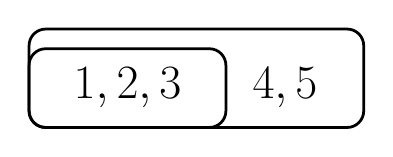
\begin{tikzpicture}
            \tikzstyle{every node}=[font=\LARGE]
            \draw [ line width=1pt , rounded corners = 6.0] (3,9) rectangle (7.25,7.75);
            \draw [ line width=1pt , rounded corners = 6.0] (3,8.75) rectangle (5.5,7.75);
            \node [font=\LARGE] at (4.25,8.25) {$1, 2, 3$};
            \node [font=\LARGE] at (6.25,8.25) {$4, 5$};
        \end{tikzpicture}

    \end{multicols}

    \subsection{Operaties op sets}
    Union $A \cup B = \{x : x \in A \lor x \in B \}$ Combineert A en B met elkaar\\
    Intersection $A \cap B = \{x : x \in A \land x \in B\}$ Het deel wat zowel in A als in B zit\\
    Complement $\overline{A} = \{x : x \not\in A\}$, alles wat niet in A zit.\\
    Difference $A\B = \{x: x \in A \land X \not\in B\}$ Alles wat in A zit, maar niet in B\\

    Zo heb je ook de \textit{powerset P(A)}, dit is een set waarin alle mogelijke subsets van A zitten: $P(A) = \{ X : X \subseteq A \}$.
    Deze heeft $n^2$ elementen, waar n het aantal elementen van set A is.

    \begin{voorbeeld}{powerset/matchsset}
        Stel je hebt een computer scherm, van 1680 x 1050, je wilt elke mogelijke configuratie van zwart/witte pixels opschrijven.
        Een set geeft aan welke pixels wit zijn, dus je wilt elke set met elke mogelijke manier van pixelcoordinaten, dat kan je zo schrijven:

        $W = \{0,1, ..., 1697\}$ voor elke X coordinaat\\
        $H = \{0,1,...,1049\}$ Voor elke Y coordinaat\\
        $W\times H = \{\{0,0\}, \{0,1\}, \{0,2\},...,\{1,0\},...\{1679,1049\}\}$ dit is een volledig wit scherm, elke pixel is gerepresentateerd in deze set\\
        $P(W\times H)$ = elke configuratie van witte pixels
    \end{voorbeeld}

    \subsection{Partities}
    Je kan een set A opdelen in meerdere sets, zoals $A_1$ en $A_2$, hier zijn de regels: $A_1 \cup A_2 = A$ en $A_1 \cap A_2 = \emptyset$
    Zo kan je A = $\mathbb{N}$ opsplitsen in $A_1$ en $A_2$ waar $A_1$ de even getallen zijn en $A_2$ de oneven getallen zijn.

    \subsection{Naive set theory}
    %TODO


    \section{Boolean algebra}
    korte notitie* in Bolean algebra is de $+$ hetzelfde als de OR operator, $\cdot$ hetzelfde als de AND operator, $^{-1}$ hetzelfde als NOT

    \subsection{monoïde}
    Monoide is een verzameling A, is niet ledig en heeft minstens 1 element e, en een binaire operator $\oplus$ %TODO: verder uitschrijven
    Een monoide heeft een nul-element, dit is een waarde die niks doet in de operatie. $x + 0 = x$, hier doet de 0 helemenaal niks, dus 0 is het 0-element in de "+" operatie.
    $x \times 1 = x$, hier is 1 het nul-element in de monoide $\times$ 1; het doet niks in de operatie.
    het is dus een neutrale waarde.

    \subsection{Bool's algebra}

    Boolean algebra heeft een paar regels:

    \begin{itemize}
        \item een set B
        \item Twee elementen $0 \in B$ en $1 \in B$, genaamd \textbf{zero} en \textbf{unit}
        \item Twee binaire operatoren $+$ en $\cdot$ som/OR en product/AND respectievelijk.
        \item Een Unaire operator $^{-1}$ de inverse genoemd ofwel NOT (kan ook als $x'$ zijn genoteerd).
    \end{itemize}

    \begin{voorbeeld}{Bewijs dat $x + x = x$}
        We willen bewijzen dat voor elke $x, x + x = x$\\
        \begin{SimpleTable}[s{.3}s{1}s{.3}]{}{}
            \TableRow{$x + x$ & $= (x + x) \cdot 1$               & Ident}
            \TableRow{        & $= (x + x)\cdot (x \cdot x^{-1})$ & Complement}
            \TableRow{        & $= x + (x \cdot x^{-1})$          & Distrobution}
            \TableRow{        & $= x + ()$                        & Complement}
            \TableRow{        & $= x$                             & Ident}
        \end{SimpleTable}
    \end{voorbeeld}

    \subsection{duality}
    Je kan voor elke vergelijking die je opschrijft een soort duale tweede vergelijking maken door hetvoglende te doen:

    \begin{itemize}
        \item 0 met 1 vervangen
        \item 1 met 0 te vervangen
        \item $+$ met $\cdot$ te vervangen
        \item $\cdot$ met $+$ te vervangen
    \end{itemize}

\end{document}